\subsection*{Probabilities}

$\E_{Y|X}[Y]=\E_{Y}[Y|X]$

$\E_{X,Y}[f(X,Y)]=\E_{X}\E_{Y|X}[f(X,Y)|X]$

$\E_{Y|X}[f(X,Y)|X]{=}\int_\mathbb{R}f(X,y)\Prob(y|X)\di y$

$\C(\X,\Y)=\E[(\X-\E[\X])(\Y-\E[\Y])] = \E[\X\Y^T]-\E[\X]\E[\Y]^T$

$\C(\mathbf{a}\X,\mathbf{b}\Y)=\mathbf{a}\C(\X,\Y)\mathbf{b}^T$

$P(A|B) = \frac{P(B|A) \cdot P(A)}{P(B)}$; $p(Z|X,\theta) = \frac{p(X,Z|\theta)}{p(X|\theta)}$

Vec. Var: $\mathbb V[\mathbf x]=\mathbb E[\mathbf x\mathbf x^T]-\mathbb E[\mathbf x]\mathbb E[\mathbf x]^T=\mathbb E[\mathbf w\mathbf w^T]-\mathbb E[\mathbf w]\mathbb E[\mathbf w]^T$

$P(x,y) = P(y|x) \cdot  P(x) = P(x|y) \cdot P(y)$
$P(x)=\sum_i P(x|y=i)P(y=i)$

\subsection*{Distributions}
$\mathcal{N}(x|\mu, \sigma^2)=\frac{\exp(-\frac{1}{2}\frac{(x-\mu)^2}{\sigma^2})}{\sqrt{2\pi\sigma^2}}$;\\
$\N(x|\mu, \Sigma)= \frac{\exp(-\frac{1}{2}(\mathbf{x}-\mu)^T\Sigma^{-1}(\mathbf{x}-\mu))}{(2\pi)^{D/2}|\Sigma|^{1/2}}$;\\
Emp.: $\hat{\Sigma} = \frac{1}{n}\sum_{i=1}^n x_i x_i^T$ (need centered data)\\
$\E[X^2]= \Sigma+ \mu\mu^T, \E[\hat{\sigma}^2]=\frac{n-1}{n}\sigma^2 $\\
$\mathrm{Exp}(x|\lambda){=}\lambda e^{-\lambda x}; \, \frac{1}{\lambda}; \, \frac{1}{\lambda^2}$\\
$\mathrm{Ber}(x|\theta){=}\theta^x (1{-}\theta)^{(1-x)}$;$ \, \theta$;$ \, \theta(1-\theta)$\\
$\mathrm{Bin}(n|\theta)=\binom{n}{x}\theta^{x}(1-\theta)^{(n-x)}$;$n\uparrow$;$n\uparrow$

\subsection*{Norms}
Frobenius norm: $\|\mathbf A\|_F = \left(\sum_{i,j}A_{i,j}^2\right)^\frac{1}{2}$

\subsection*{Jensen}
$\phi(\E)\leq \E[\phi]$; $\phi$ convex (reversed if concave:)$\E[\min]\leq \min\E$;$\E[\log]\leq\log\E$
\subsection*{Convex, smooth $f(x)$}
$f''(x) > 0 \Leftrightarrow x_1,x_2 \in \mathbb{R}, \lambda \in [0,1]:
f(\lambda x_1 + (1-\lambda) x_2) \leq \lambda f(x_1) + (1-\lambda) f(x_2)$\\
strong: 
$f(x+y)\geq f(x)+\nabla f(x)\cdot y+\frac{\mu}{2}\| y\|$\\
L-smooth: $\| \nabla f(x)-\nabla f(x+y)\|\leq L\|y\|$, $f\in C^2: f(x+y)\leq f(x)+\nabla f(x)\cdot y+\frac{L}{2}\| y\|^2$;
$\mu \preceq \nabla^2f \preceq L$


\subsection*{Pos semi-definite mat $M \in \mathbb{R}^{n\times n}$}
$\forall x \in \mathbb{R}^n: x^TMx \geq 0 \Leftrightarrow$ eigenvalues $\lambda_i\geq 0$
\subsection*{Completing squares}
$x^{\mathrm {T} }Ax+x^{\mathrm {T} }b+c=(x-h)^{\mathrm {T} }A(x-h)+k$ \\
$A=A^{\mathrm {T} }:\quad h=-{\frac {1}{2}}A^{-1}b,\quad k=c-{\frac {1}{4}}b^{\mathrm {T} }A^{-1}b$\\
$h=-(A+A^{\mathrm {T} })^{-1}b,\quad k=c-h^{\mathrm {T} }Ah=c-b^{\mathrm {T} }(A+A^{\mathrm {T} })^{-1}A(A+A^{\mathrm {T} })^{-1}b$\\
$\mathbf{x}^T\mathbf{A}\mathbf{x}-2\mathbf{b}^T\mathbf{x} = (\mathbf{x}-\mathbf{A}^{-1}\mathbf{b})^T\mathbf{A}(\mathbf{x}-\mathbf{A}^{-1}\mathbf{b})-\mathbf{b}^T\mathbf{A}^{-1}\mathbf{b}$;\\
$ax^{2}+bx+c=a(x+\frac{b}{2a})^{2}+c-\frac{b^2}{4a}$

\subsection*{Derivatives}

$\frac{\text{d}}{\text{d}\mathbf x}\mathbf x^T\mathbf B=\mathbf B = \frac{\text{d}}{\text{d}\mathbf x}\mathbf B\mathbf x$

$\frac{\text{d}}{\text{d}\mathbf x}\mathbf x^T\mathbf b=\mathbf b$

$\frac{\text{d}}{\text{d}\mathbf x}\mathbf x^T\mathbf x=2\mathbf x$

$\frac{\text{d}}{\text{d}\mathbf x}\mathbf x^T\mathbf B \mathbf x=2\mathbf B\mathbf x$

$\frac{\text{d}}{\text{d}\mathbf B}\mathbf x^T\mathbf B \mathbf x=\mathbf x^T\mathbf x$


$\nabla_v f(w)=\nablaf(w)^T v=\lim_{\lambda \rightarrow 0}\frac{f(w+\lambda v)-f(w)}{\lambda}$

$\nabla_\x\log(1+\exp(-\alpha x))=\frac{-\alpha}{1+\exp(\alpha x)}$
$\frac{\partial}{\partial \mathbf{x}}(\mathbf{x}^\top \mathbf{A}\mathbf{x}) = (\mathbf{A}^\top + \mathbf{A})\mathbf{x} (= 2\mathbf{A}\x$ if symm) \quad\\
$\frac{\partial}{\partial \mathbf{x}}(\mathbf{b}^\top \mathbf{A}\mathbf{x}) = \mathbf{A}^\top \mathbf{b}$ \quad
$\frac{\partial}{\partial \mathbf{X}}(\mathbf{c}^\top \mathbf{X} \mathbf{b}) = \mathbf{c}\mathbf{b}^\top$ \quad
$\frac{\partial}{\partial \mathbf{x}}(\| \mathbf{x}-\mathbf{b} \|_2) = \frac{\mathbf{x}-\mathbf{b}}{\|\mathbf{x}-\mathbf{b}\|_2}$

$\frac{\partial}{\partial \mathbf{x}}(\| \mathbf{x}-\mathbf{b} \|_2^2) = 2(\mathbf x -\mathbf b)$

$\frac{\partial}{\partial \mathbf{x}}(\|\mathbf{x}\|^2_2) = \frac{\partial}{\partial \mathbf{x}} (\mathbf{x}^\top \mathbf{x}) = 2\mathbf{x}$ \quad
\\$\frac{\partial}{\partial \mathbf{X}}(\|\mathbf{X}\|_F^2) = 2\mathbf{X}$  \quad \quad
$\frac{\partial}{\partial \mathbf{x}}||\mathbf{x}||_1 = \frac{\mathbf{x}}{|\mathbf{x}|}$ \\
$\frac{\partial}{\partial \mathbf{x}}(\|\mathbf{Ax - b}\|_2^2) = \mathbf{2(A^\top Ax-A^\top b)}$ \quad
$\frac{\partial}{\partial \mathbf{X}}(|\mathbf{X}|) = |\mathbf{X}|\cdot \mathbf{X}^{-1}$ $\quad |X| = 1 / |X^{-1}|$\\
$\frac{\partial}{\partial x}(\mathbf{Y}^{-1}) = -\mathbf{Y}^{-1} \frac{\partial\mathbf{Y}}{\partial x} \mathbf{Y}^{-1}$

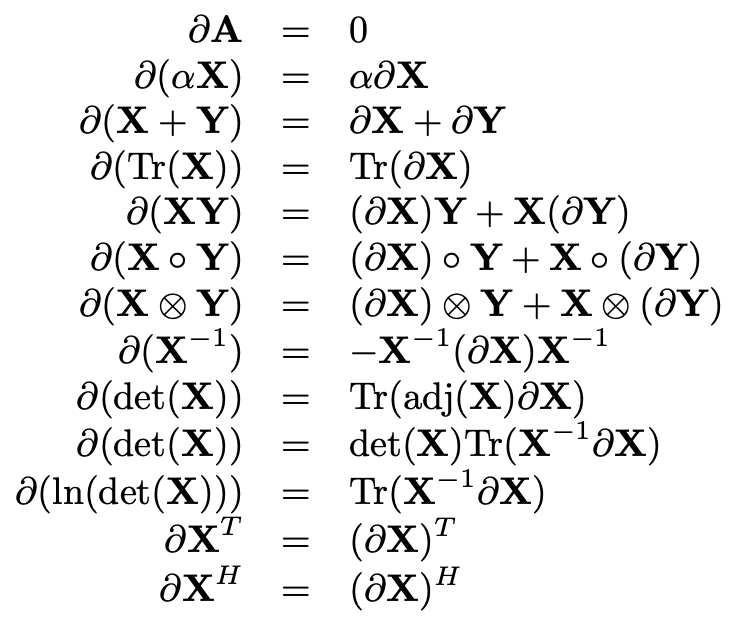
\includegraphics[width=.7\columnwidth]{src/matrix_deriv.png}

\subsection*{Matrices}

Cauchy-Schwarz: $\mathbf a^\top\mathbf b \leq \|\mathbf a\|_2\|\mathbf b\|_2$

Norms: $\mathbf w^\top\mathbf w=\|\mathbf w\|_2^2$, $\mathbf w^\top\text{sgn}(\mathbf w)=\sum_i |x_i|=\|\mathbf w \|_1$

Traces: $\text{Tr}(A+B)=\text{Tr}(A)+\text{Tr}(B)$, $\text{Tr}(AB)=\text{Tr}(BA)$, $\mathbf{a}^T \mathbf a = \text{Tr}(\mathbf{aa}^T)$, $\mathbf x^T\mathbf M\mathbf x=\text{Tr}(\mathbf x^T\mathbf M\mathbf x)$, $\mathbf x^T\mathbf y = \text{Tr}(\mathbf{yx}^T)$, if $\mathbf A$ s.p.d then $\text{Tr}(\mathbf A)\geq 0$.

Vector projection $\mathbf a$ to $\mathbf b$: $\frac{\mathbf a^\top \mathbf b}{\|\mathbf b\|^2}\mathbf b$

\iffalse
\subsection*{Parametric vs. Nonparametric}
\textbf{Parametric}: have finite set of parameters. 
e.g. linear regression, linear perceptron\\
\textbf{Nonparametric}: grow in complexity with the size of the data, more expressive.
e.g. k-NN
\fi